\section{Experiments}
\label{sec:experiments}



We conduct our experiments using language models that are commonly employed in practical applications. Each dataset (details provided below) is partitioned into two non-overlapping subsets of 3,000 samples each, and a separate model is fine-tuned on each subset. In this setup, every training example is treated as potentially copyright-protected. To evaluate the copyright protection capabilities of CP-Fuse, we simulate an extreme scenario by overfitting the models to the subsets by fine-tuning them for 50 epochs (see Appendix~\ref{app:implementation}). As a result, the base models strongly memorize the data, representing a challenging setting where they are prone to reproducing a significant amount of training samples.


\paragraph{Datasets and Models} We perform fine-tuning using four datasets, each associated with a specific task. \textbf{(I) Abstract Generation:} We fine-tune the LLaMa2 7B model \citep{touvron2023llama} on a dataset of abstracts from math papers (\texttt{MathAbstracts}) \citep{zhang2024autonomous}, using each paper's title as the prompt. 
\textbf{(II) Story-telling:} We also fine-tune LLaMa2 on the story-generation dataset \texttt{WritingPrompts} \citep{fan2018hierarchical}, using the topic of the story as the prompt. \textbf{(III) Code Generation:} We fine-tune the StarCoder 7B model \citep{li2023starcoder} on an instructional dataset for Python (\texttt{Python instructions}), where the prompts are natural language descriptions of tasks and the responses are Python solutions. \textbf{(IV) Code Generation with Unit Tests:} We fine-tune again a StarCoder model on the \texttt{APPS} dataset \citep{hendrycksapps2021}, which also consists of natural language problems and Python solutions, but additionally incorporates unit tests to assess code generation quality. For this task, the models are further evaluated on the \texttt{MBPP} \citep{austin2021program} and \texttt{HumanEval} \citep{chen2021evaluating} datasets, which also include unit tests. Both code and text-based tasks represent settings where copyright infringement is a concern \citep{yu2023codeiipprompt, henderson2023foundation}. We provide additional information on the datasets in \Cref{app:datasets}.

\paragraph{Copyright-infringement metrics} We use a comprehensive set of metrics to evaluate potential copyright infringement. The models are prompted with the initial part of samples from their fine-tuning splits. We then compare the generated outputs against the original samples. For each metric, we report the average value above the 95th percentile. This focus on high percentiles is motivated by the legal concern that models might reproduce only a few long text extracts in a real-world scenario.




To measure \textit{exact memorization}, we use the average Exact Matching (EM) length and the Infringement Count (IC) for substrings exceeding 160 characters (in \Cref{app:more_copyright}). While the former is widely recognized in the literature as a clear indicator of copyright infringement in both text and code \citep{lee2021deduplicating, karamolegkou2023copyright, carlini2023quantifying, yu2023codeiipprompt}, the latter count with a threshold at 160 is consistent with regulatory guidelines \citep{mueller2024llms}.

For \textit{approximate memorization}, we report the BLEU score and normalized Levenshtein distance in the main text, with additional results for ROUGE-L score, METEOR score, Jaccard similarity, cosine similarity, and semantic similarity in \Cref{app:more_copyright}. These metrics are well-established in the literature, see e.g., \citep{ippolito2023preventing, huang2023privacy, chen2024copybench}. For the \texttt{Python instructions} dataset, we also report specialized metrics obtained from two state-of-the-art plagiarism detection tools: JPlag \citep{prechelt2002finding} and Dolos \citep{maertens2022dolos}. We refer to \Cref{app:metrics_copy} for full details on the implementation of the copyright-infringement metrics.


\paragraph{Utility metrics} For text-based tasks, we evaluate \textit{fluency} using the Prometheus-v2 model \citep{kim2024prometheus}, which serves as a judge for the stories generated by models fine-tuned on \texttt{WritingPrompts}. Model-based fluency metrics have been shown to closely align with human evaluations \citep{liu2023g, sottana2023evaluation}, particularly for the \texttt{WritingPrompts} dataset \citep{chiang2023can}. Prometheus-v2 has also demonstrated consistent alignment with human annotators and GPT-4 \citep{kim2024prometheus}. We use the five-point rubric detailed in \Cref{app:rubric}. For code-based tasks, we use the \texttt{APPS}, \texttt{MBPP}, and \texttt{HumanEval} datasets, which include unit tests that allow for the computation of the \textit{pass@1 score} \citep{chen2021evaluating}. We report the utility metrics in a separate test set comprising 500 prompts for each dataset. Refer to \Cref{app:metrics_utility} for full details on the implementation.




\paragraph{Comparison with inference-time baselines} 
We compare CP-Fuse against three protection measures that intervene at the inference stage. We report results using token-wise $\cpdelta$ \citep{vyas2023provable}, with KL divergence as $\Delta$; a system-mode self-reminder method \citep{xie2023defending}, where the model is explicitly instructed to avoid regurgitating memorized data; and MemFree decoding \citep{ippolito2023preventing}, which prevents 10-gram copying from the training data by using a Bloom filter. Implementation details for these baselines are provided in \Cref{app:baselines}. For CP-Fuse, we construct the grid by discretizing the interval $[0, 2)$ into 10 steps, and $[2, 10]$ into 9 steps (see ablation studies in \Cref{app:ablation_grid}). Greedy decoding is used for all experiments presented in the main text, with results from temperature sampling—leading to equivalent conclusions—provided in \Cref{app:sampling}. Additionally, we conduct experiments combining three models instead of two in \Cref{app:multiple_models}.

\begin{table*}[t!]
\caption{Copyright-infringement metrics \textbf{averaged at the 95th percentile} for the \texttt{Python instructions}, \texttt{MathAbstracts}, and \texttt{WritingPrompts} datasets across fine-tuning splits. We present results for the overfitted models, Self-reminder prompting (SystemPrompt), MemFree, $\cpdelta$, and CP-Fuse. Metrics include Exact Matching (EM), BLEU score (BLE), Levenshtein Distance (LEV), and code plagiarism score JPlag (JP). Arrows indicate the preferred direction: $\uparrow$ (higher is better) and $\downarrow$ (lower is better). We highlight in \textbf{bold} the best method for each split and metric.}
\centering
% \footnotesize
\begin{tabular}{l l|c c|c c c|c c c}
\toprule
\textbf{Model} & \textbf{Split} & \textbf{EM}\textsuperscript{$\downarrow$} & \textbf{JP}\textsuperscript{$\downarrow$} & \textbf{EM}\textsuperscript{$\downarrow$} & \textbf{BLE}\textsuperscript{$\downarrow$} & \textbf{LEV}\textsuperscript{$\uparrow$} & \textbf{EM}\textsuperscript{$\downarrow$} & \textbf{BLE}\textsuperscript{$\downarrow$} & \textbf{LEV}\textsuperscript{$\uparrow$} \\
\midrule
& & \multicolumn{2}{c|}{\texttt{Python inst.}} & \multicolumn{3}{c|}{\texttt{MathAbstracts}} & \multicolumn{3}{c}{\texttt{WritingPrompts}} \\
\midrule
\multirow{2}{*}{\makecell{Overfit \\ Split 1}} 
& Split 1 & 1469.80 & 1.00 & 1397.68 & 1.00 & 0.00 & 1316.24 & 1.00 & 0.00 \\
& Split 2 & 44.60   & 0.01 & 31.00   & 0.01 & 0.70 & 22.59 & 0.03 & 0.71 \\
% & Test    & 54.38   & 0.02 & 28.76   & 0.04 & 0.71 & 16.89 & 0.02 & 0.71 \\
\midrule
\multirow{2}{*}{\makecell{Overfit \\ Split 2}} 
& Split 1 & 42.64   & 0.01 & 42.12   & 0.08 & 0.68 & 26.11 & 0.02 & 0.70 \\
& Split 2 & 1393.88 & 0.99 & 1570.88 & 1.00 & 0.00 & 1141.88 & 1.00 & 0.00 \\
% & Test    & 53.26   & 0.01 & 37.48   & 0.07 & 0.69 & 23.60 & 0.03 & 0.71 \\
\midrule
\midrule
\multirow{2}{*}{\makecell{System \\ Prompt}} 
% & Split 1 & 1360.68 & 1.00 & 1022.72 & 0.99 & 0.00 & 1518.36 & 1.00 & 0.00 \\
% & Split 2 & 1373.16 & 0.99 & 1005.20 & 1.00 & 0.00 & 1492.20 & 1.00 & 0.00 \\
% & Test    & 72.44   & \textbf{0.01} & 36.44 & \textbf{0.06} & 0.69 & 14.58 & \textbf{0.02} & \textbf{0.71} \\
& Split 1 & \WorstCell{1360.68} & \WorstCell{1.00} & \WorstCell{1022.72} & \WorstCell{0.99} & \WorstCell{0.00} & \WorstCell{1118.36} & \WorstCell{1.00} & \WorstCell{0.00} \\
& Split 2 & \WorstCell{1373.16} & \WorstCell{0.99} & \WorstCell{1005.20} & \WorstCell{1.00} & \WorstCell{0.00} & \WorstCell{1092.20} & \WorstCell{1.00} & \WorstCell{0.00} \\
% & Test    & \MiddleGreenCell{72.44}   & \BestCell{0.01} & \AlmostBestCell{36.44} & \BestCell{0.06} & \AlmostBestCell{0.69} & \AlmostBestCell{14.58} & \BestCell{0.02} & \BestCell{0.71} \\
\midrule
\multirow{2}{*}{MemFree} 
& Split 1 & \MiddleYellowCell{165.48}  & \WorstCell{0.99} & \MiddleYellowCell{111.12}  & \MiddleYellowCell{0.23} & \MiddleYellowCell{0.53} & \MiddleYellowCell{63.84} & \MiddleYellowCell{0.20} & \MiddleYellowCell{0.55} \\
& Split 2 & \MiddleYellowCell{157.36}  & \WorstCell{0.96} & \MiddleYellowCell{99.40}   & \MiddleYellowCell{0.22} & \MiddleYellowCell{0.53} & \MiddleYellowCell{59.04} & \MiddleYellowCell{0.19} & \MiddleYellowCell{0.55} \\
% & Test    & \AlmostBestCell{52.33}   & \BestCell{0.01} & \AlmostBestCell{39.32}   & \AlmostBestCell{0.07} & \BestCell{0.70} & \BestCell{14.25} & \BestCell{0.02} & \BestCell{0.71} \\
\midrule
\multirow{2}{*}{$\cpdelta$} 
& Split 1 & \MiddleRedCell{273.20}  & \WorstCell{1.00} & \MiddleRedCell{341.60}  & \MiddleRedCell{0.58} & \MiddleRedCell{0.30} &  \MiddleGreenCell{37.40} &  \MiddleGreenCell{0.05} & \BestCell{0.70} \\
& Split 2 & \MiddleRedCell{284.80}  & \WorstCell{0.99} & \MiddleYellowCell{162.80}  & \MiddleYellowCell{0.30} & \MiddleYellowCell{0.51} &  \MiddleGreenCell{31.29} &  \MiddleGreenCell{0.04} & \BestCell{0.70} \\
% & Test    & \AlmostBestCell{57.50}   & \BestCell{0.01} & \AlmostBestCell{39.91}   & \AlmostBestCell{0.07} & \AlmostBestCell{0.67} &  \AlmostBestCell{16.22} &  \BestCell{0.02} & \BestCell{0.71} \\
\midrule
\multirow{2}{*}{\makecell{CP-Fuse \\(Ours)}} 
& Split 1 & \BestMiddleGreenCell{69.58}   & \BestCell{0.03} & \BestCell{55.54}   & \BestCell{0.14} & \BestCell{0.62} & \BestCell{27.55} & \BestCell{0.02} & \BestCell{0.70} \\
& Split 2 & \BestMiddleGreenCell{68.04}   & \BestCell{0.03} & \BestCell{48.74}   & \BestCell{0.14} & \BestCell{0.63} & \BestCell{25.50} & \BestCell{0.03} & \BestCell{0.70} \\
% & Test    & \BestCell{48.80}   & \BestCell{0.01} & \BestCell{35.59}   & \AlmostBestCell{0.07} & \AlmostBestCell{0.68} & \AlmostBestCell{16.04} & \BestCell{0.02} & \BestCell{0.71} \\
\bottomrule
\end{tabular}
\label{tab:results_copyright}
\end{table*}

\paragraph{Combining CP-Fuse with training-time strategies} In \Cref{sec:wraping_exps}, we apply CP-Fuse on top of models trained with the goldfish loss \citep{hans2024like}, setting the dropout frequency to $k=16$. In \Cref{app:early_stopped}, we use CP-Fuse to wrap early-stopped models, a simple way of preventing memorization. We stop fine-tuning after 3 epochs.



\subsection{Preventing copyright infringement with CP-Fuse}
\label{sec:exp_copyright}
\Cref{tab:results_copyright} presents the copyright-infringement metrics for the overfitted models, the baselines, and CP-Fuse across fine-tuning splits. CP-Fuse substantially reduces verbatim regurgitation in both code and text tasks. Specifically, CP-Fuse decreases exact matches by more than a factor of 25 compared to the overfitted models and consistently outperforms the baselines. In particular, the system-mode self-reminder (SystemPrompt) fails to prevent the reproduction of memorized samples, potentially due to the override of safety fine-tuning during our fine-tuning. MemFree noticeably reduces the length of memorized text segments; however, it still reproduces segments twice as long as those produced by CP-Fuse. A quick inspection of MemFree outputs also reveals that it often avoids exact copying simply by inserting spaces or spelling mistakes (refer to \Cref{app:comparison_memfree} for examples). Finally, $\cpdelta$ still generates long text segments that exactly match the training data, often 4 to 7 times longer than those produced by CP-Fuse. These segments frequently exceed the legal 160-character threshold \citep{mueller2024llms}, while such infringements almost entirely disappear with our method (refer to \Cref{app:more_copyright}).





The approximate memorization metrics further support these observations. We observe a consistent improvement with CP-Fuse compared to the overfitted models, also offering better protection than the baselines. Notably, CP-Fuse achieves near ``non-plagiarism'' on the code task, as the JPlag tool detects almost no copying in the generated code, while it clearly indicates infringement for all baselines. 

These findings demonstrate the effectiveness of our method in preventing both verbatim and quasi-verbatim reproduction of memorized training material. Additional metrics supporting these conclusions are provided in \Cref{app:more_copyright}. Furthermore, experiments using temperature sampling decoding, detailed in \Cref{app:sampling}, yield equivalent conclusions. We also explore combining three models instead of two in \Cref{app:multiple_models}, which provides further improvement in the memorization metrics.


\paragraph{Comparison between CP-Fuse and $\cpdelta$} We now provide a more detailed comparison between our method and $\cpdelta$. \Cref{fig:combined} shows histograms illustrating the distribution of exact matches generated by both methods. We observe a significantly heavier-tailed distribution for $\cpdelta$, which consistently reproduces longer verbatim text segments than CP-Fuse and is therefore more likely to infringe on copyright. For instance, the longest exact match for CP-Fuse in the abstracts task is 73 characters, whereas the 95th percentile for $\cpdelta$ is 342 characters, with the longest match exceeding 500 characters. These results highlight the importance of adaptively setting the weights based on sequence history when combining the models to ensure effective copyright protection. We provide examples of extracts produced by both methods for different datasets in \Cref{app:comparison_cpdelta}.

\begin{figure*}[t!]
    \centering
    \begin{subfigure}[b]{0.48\textwidth}
        \centering
        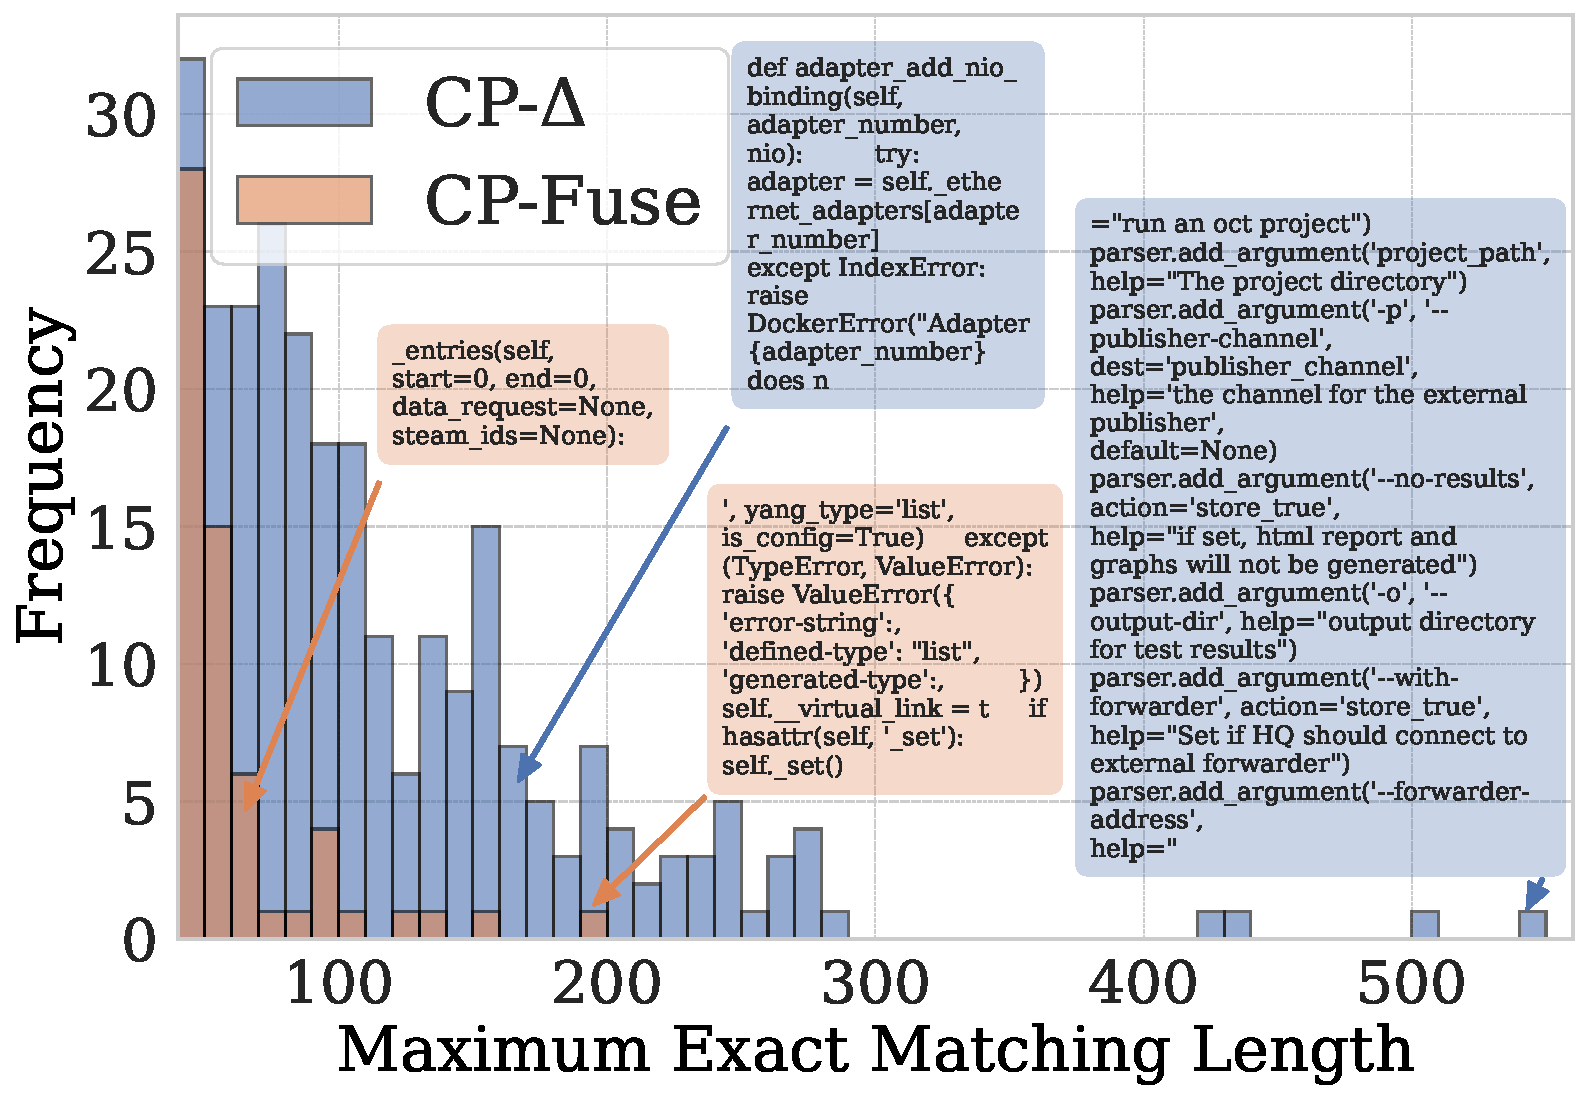
\includegraphics[width=\textwidth]{figures/python_starcoder_cut.pdf}
        \caption{\texttt{Python instructions}}
        \label{fig:python_starcoder}
    \end{subfigure}%
    \begin{subfigure}[b]{0.48\textwidth}
        \centering
        \includegraphics[width=\textwidth]{figures/abstracts_LLaMa2_cut.pdf}
        \caption{\texttt{MathAbstracts}}
        \label{fig:abstracts_LLaMa}
    \end{subfigure}
    \caption{Histogram of exactly matched substring lengths (above 40 characters) generated by CP-$\Delta$ and CP-Fuse for (a) the \texttt{Python instructions} and (b) the \texttt{MathAbstracts} datasets. We show the longest substring and one randomly sampled match above 40 characters.}
    \label{fig:combined}
    
\end{figure*}






\subsection{Utility evaluation for code generation and story-telling}
\label{sec:utility_exps}

\begin{table}[t!]
\caption{Utility metrics across datasets. Pass@1 is reported for \texttt{APPS}, \texttt{MBPP}, and \texttt{HumanEval} (\texttt{HE}); Fluency is reported for \texttt{WritingPrompts} (\texttt{WP}). Arrows indicate the preferred direction.}
\centering
\begin{tabular}{lcccc}
\toprule
\textbf{} & \multicolumn{3}{c}{\textbf{Pass@1} $\uparrow$} & \textbf{Fluency} $\uparrow$ \\
\cmidrule(lr){2-4} \cmidrule(lr){5-5}
& \texttt{APPS} & \texttt{MBPP} & \texttt{HE} & \texttt{WP} \\
\midrule
Overfit Split 1 & 0.43 & 0.44 & 0.29 & 2.17  \\
Overfit Split 2 & 0.42 & 0.44 & 0.28 & 2.16  \\
\midrule
SystemPrompt & 0.41 & 0.43 & 0.29 & 2.00  \\
MemFree & 0.32 & 0.41 & 0.24 & 1.70  \\
$\cpdelta$ & 0.45 & 0.46 & 0.29 & 2.15 \\
CP-Fuse (Ours) & 0.47 & 0.43 & 0.28 & 2.17  \\
\bottomrule
\end{tabular}
\label{tab:results_utility}
\end{table}


\begin{figure}[b!]
    \centering
    \hspace*{-3mm}
    \begin{tabular}{cc}
        % Left Column: Error Type 1
        \begin{tcolorbox}[colback=orange!10, colframe=black!75, title=Example 1: Syntax Error (NameError), width=0.50\textwidth, halign=center]
            \centering 
            \begin{tcolorbox}[colback=gray!10, colframe=black!75, title= \quad  \quad StarCoder + MemFree, width=\textwidth, left=2mm, right=2mm, arc=2.5mm, top=-2mm, bottom=-2mm]
            \vspace{-3.5mm}
            
\includegraphics[height=1em]{figures/robot.pdf} 
            \begin{lstlisting}[language=Python, basicstyle=\ttfamily\scriptsize]
def checkRecord(self , s):
    count = 0 
    for i in range(0,len((*@\textcolor{orange}{\underline{S}}@*))):
        if S[i] == 'A':
            count += 1 
            if count == 2:
                return False 
        elif i >= 2 and S[i]==S[i-2]:
            return False
    
    return True
            \end{lstlisting}
            \end{tcolorbox}
            \vspace*{3.4mm}
            \begin{tcolorbox}[colback=red!10, colframe=red!75, title=
            % \emoji{beetle} 
            \quad \quad Compilation Output, width=\textwidth, left=2mm, right=2mm, arc=2.5mm, top=-2mm, bottom=-2mm]
            \vspace{-4mm}
            
\includegraphics[height=1.2em]{figures/bug.pdf}
            \begin{lstlisting}[basicstyle=\ttfamily\scriptsize] 
Traceback (most recent call last):
  File "x.py", line 4, in checkRecord
    for i in range(0,len(S)):  
NameError: name 'S' is not defined
            \end{lstlisting}
            \end{tcolorbox}
        \vspace*{3.0mm}
        \end{tcolorbox}
                    \hspace*{-4mm} % Adjust horizontal spacing
        & % Separator for side-by-side boxes
        
        % Right Column: Error Type 2
        \begin{tcolorbox}[colback=orange!10, colframe=black!75, title=Example 2: Logic Error, width=0.50\textwidth, halign=center]
            \centering % Ensure content is centered
            \begin{tcolorbox}[colback=blue!10, colframe=blue!75, title=
            % \emoji{woman-scientist-dark-skin-tone} 
            \quad \quad Prompt, width=\textwidth, left=2mm, right=2mm, arc=2.5mm, top=-2mm, bottom=-2mm]
            \vspace{-4.5mm}
            
\includegraphics[height=1.2em]{figures/scientist.pdf}
\begin{lstlisting}[basicstyle=\ttfamily\scriptsize]
Write a Python function that counts 
how often a character appears within
a string, case insensitive.
\end{lstlisting}
            \end{tcolorbox}
            % \vspace{4mm}
            \begin{tcolorbox}[colback=gray!10, colframe=black!75, title=
            % \emoji{robot}
 \quad \quad StarCoder + MemFree, width=\textwidth, left=2mm, right=2mm, arc=2.5mm, top=-2mm, bottom=-2mm]
             \vspace{-3.5mm}
            
\includegraphics[height=1em]{figures/robot.pdf}
            \begin{lstlisting}[language=Python, basicstyle=\ttfamily\scriptsize]
def count_char(s, c):
    return s.lower().count(c.(*@\textcolor{orange}{\underline{upper()}}@*))
            \end{lstlisting}
            \end{tcolorbox}
            \begin{tcolorbox}[colback=gray!5, colframe=black!40, title=
            % \emoji{robot}
 \quad \quad StarCoder + CP-Fuse, width=\textwidth, left=2mm, right=2mm, arc=2.5mm, top=-2mm, bottom=-2mm]
             \vspace{-3.5mm}
            
\includegraphics[height=1em]{figures/robot.pdf}
            \begin{lstlisting}[language=Python, basicstyle=\ttfamily\scriptsize]
def count_char(s, c):
    a = s.lower()
    b = c.lower()
    return a.count(b)
            \end{lstlisting}
            \end{tcolorbox}
            % \vspace{4mm}
            \begin{tcolorbox}[colback=green!10, colframe=yellow!20!green!100, title=
            % \emoji{check-mark} 
            \quad \quad Correct Answer, width=\textwidth, left=2mm, right=2mm, arc=2.5mm, top=-2mm, bottom=-2mm]
                        \vspace{-3.5mm}
            
\includegraphics[height=1em]{figures/check.pdf}
            \begin{lstlisting}[language=Python, basicstyle=\ttfamily\scriptsize]
def count_char(s, c):
    return s.lower().count(c.lower())  
            \end{lstlisting}
            \end{tcolorbox}      

             % \vspace*{2mm}
        \end{tcolorbox}
        
    \end{tabular}
    
\caption{Examples of typical errors in code generated by MemFree for the \texttt{APPS} dataset. The \textcolor{orange}{\underline{highlighted}} characters indicate the code affected by filtering, leading to errors. On the left, MemFree changes a variable name, resulting in a syntax error. On the right, MemFree alters the logic of the code, producing incorrect output, whereas CP-Fuse successfully solves the problem.}

    \label{fig:memfree_code_error_comparison}
\end{figure}


The success of our method in preventing the exact and approximate reproduction of memorized training samples raises the question of whether it still generates useful text and code for solving the task at hand.  In \Cref{tab:results_utility}, we present the results for the considered utility metrics, pass@1 for code-based tasks and fluency for story-telling writing, on the test splits not seen during fine-tuning. We observe that CP-Fuse produces code that is as accurate as that generated by the overfitted models, passing a similar proportion of unit tests. Additionally, the stories generated based on the \texttt{WritingPrompts} dataset achieve the same level of fluency as those produced by copyright-infringing models. All baselines perform similarly, with the notable exception of MemFree, which consistently underperforms.

We further validate the high quality of text and code produced by our method with examples of its outputs in \Cref{app:comparison_cpdelta}. For the code tasks, CP-Fuse generates code that is significantly different from the original, effectively solving the tasks while often incorporating exception handling and additional features. For the text tasks, it produces well-written stories and coherent abstracts that also differ notably from the reference. 

\paragraph{Comparison between CP-Fuse and MemFree} Filtering approaches like MemFree are susceptible to hallucinations \citep{ippolito2023preventing, liu2024shield}. This issue is particularly problematic in code generation, where even minor changes, such as modifying variable names or introducing typos, can result in incorrect code. As a result, MemFree underperforms on the \texttt{APPS} dataset due to the lengthy Python solutions, which increase the likelihood of hallucinations and, consequently, syntax and logic errors. We provide two examples in \Cref{fig:memfree_code_error_comparison}. The \texttt{MBPP} and \texttt{HumanEval} datasets, with their shorter problems, are less affected by this issue. A similar problem arises in the \texttt{WritingPrompts} dataset, where alterations in the decoding process can lead to grammatical and spelling errors or cause the model to deviate from the intended topic (see \Cref{app:comparison_memfree} for examples). In contrast, CP-Fuse generates tokens that are consistent with at least one of the two combined models.
% ; when both models are properly fine-tuned, CP-Fuse produces outputs that are useful and significantly different from the training set.









\subsection{CP-Fuse as a wrapper of other protection methods}
\label{sec:wraping_exps}

In this section, we demonstrate how CP-Fuse can be combined with other training-time methods to enhance protection. Specifically, we apply CP-Fuse on top of models fine-tuned on the \texttt{WritingPrompts} dataset using the goldfish loss \citep{hans2024like}, a recently proposed technique designed to mitigate memorization during training. As presented in \Cref{tab:results_wrapping}, integrating CP-Fuse results in further improvements in both the exact match and BLEU score. We also conduct similar experiments in \Cref{app:early_stopped}, where CP-Fuse is applied on top of early-stopped models—another strategy aimed at reducing memorization during training. 

\begin{figure*}[b!]
\centering
\begin{subfigure}[t!]{0.50\textwidth}
    \centering
    \begin{tabular}{l l|c c}
    \toprule
    \textbf{Model} & \textbf{Split} & \textbf{EM}\textsuperscript{$\downarrow$} & \textbf{BLE}\textsuperscript{$\downarrow$} \\
    \midrule
    \multirow{2}{*}{GL Split 1}
    & Split 1 & 84.68 & 0.11  \\
    & Split 2 & 21.79 & 0.03  \\
    \midrule
    \multirow{2}{*}{GL Split 2} 
    & Split 1 &  19.11 & 0.02 \\
    & Split 2 &  120.28 & 0.16 \\
    \midrule
    \midrule
    \multirow{2}{*}{CP-Fuse} 
    & Split 1 & 20.68 & 0.03  \\
    & Split 2 & 25.50 & 0.03 \\
    \bottomrule
    \end{tabular}
    \caption{Wrapping experiments with GL loss}
    \label{tab:results_wrapping}
\end{subfigure}%
\begin{subfigure}[t!]{0.50\textwidth}
    \centering
    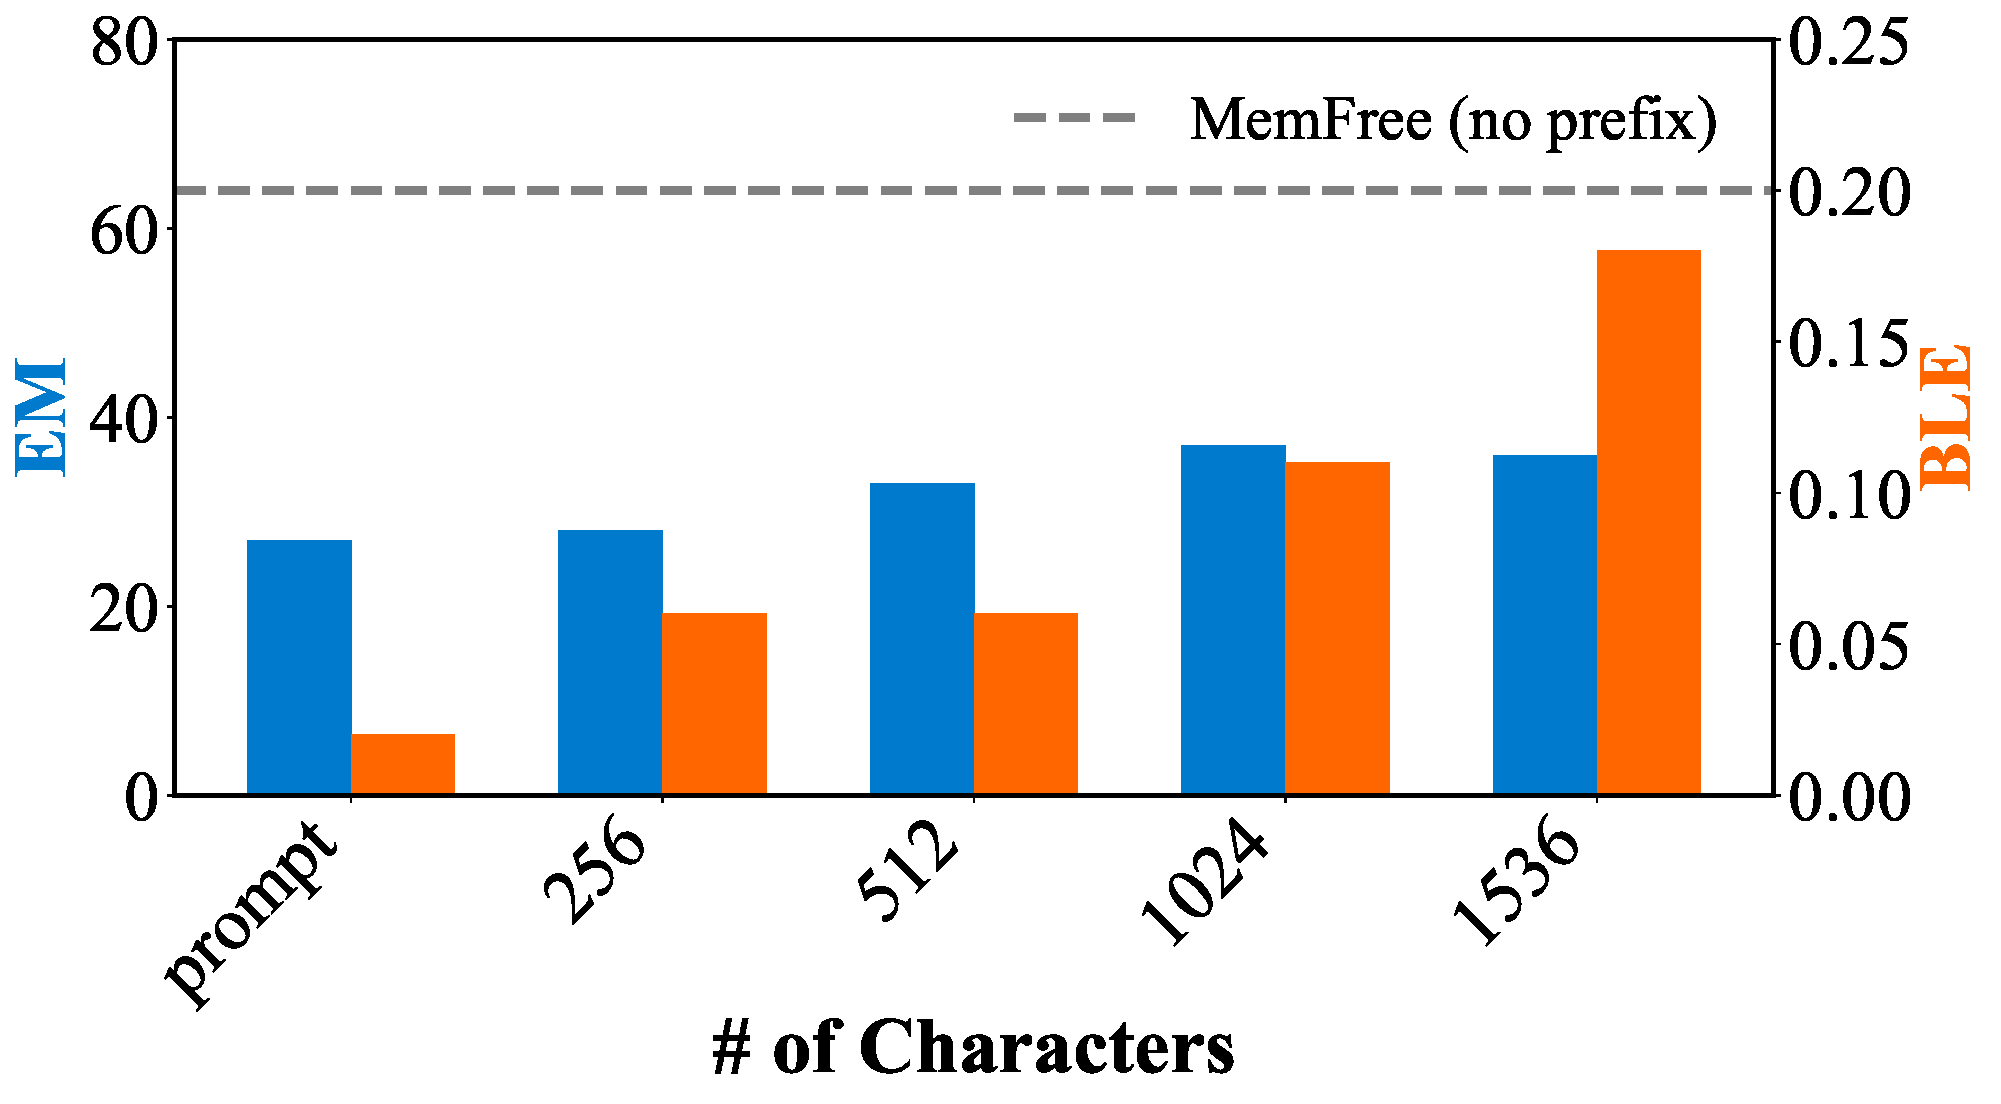
\includegraphics[width=\textwidth]{figures/plot_attacks.pdf}
    \caption{Prefix prompting experiments}
    \label{fig:plot_attacks}
\end{subfigure}
\caption{Metrics for copyright infringement, exact matching (EM), and BLEU score (BLE) in the \texttt{WritingPrompts} dataset for (a) models trained with goldfish loss (GL) and CP-Fuse as a wrapper, and (b) the effect of the prefix length on CP-Fuse applied to overfitted models in the split 1.}
\end{figure*}
\subsection{Robustness of CP-Fuse under prefix prompting  extractions}
\label{sec:attacks}

Previous sections have shown that our method effectively reduces regurgitation without sacrificing utility. In this final section, we evaluate the robustness of CP-Fuse against \textit{prefix prompting} extractions using the \texttt{WritingPrompts} dataset. We assume a \textit{threat model} where an adversary has black-box access to CP-Fuse, which wraps two potentially copyright-infringing models. The attacker has access to the prompts used during fine-tuning, as well as a prefix of the original story, and their \textit{goal} is to have CP-Fuse regurgitate a story memorized by one of the base models. We study the impact of increasing the prefix length on the exact match (EM) and BLEU score of the generated outputs. The results in \Cref{fig:plot_attacks} show that CP-Fuse remains robust as the prefix length increases. Specifically, exact matching remains relatively stable, while there is a slight increase in the BLEU score; however, it is still significantly smaller than that observed in the overfitted models and baselines (\Cref{tab:results_copyright}). In \Cref{app:attacks}, we visualize the stories generated by CP-Fuse and show how they evolve given short and long prefix lengths. CP-Fuse consistently produces outputs that differ from the reference, thanks to its balancing mechanism that prevents any single model from dominating the generation process.






\section{Conclusions}

In this paper, we introduced CP-Fuse, a simple yet highly effective algorithm for copyright protection based on model fusion. We first demonstrated that CP-Fuse satisfies key properties for preventing the reproduction of memorized training samples. Additionally, we provided extensive evidence of its effectiveness in challenging scenarios involving overfitted models, where CP-Fuse significantly reduced the regurgitation of protected materials, outperforming other inference-time baselines without compromising the quality of the generated code and text. The versatility of CP-Fuse was further demonstrated through its seamless integration with other training-time techniques that mitigate memorization. Finally, we showcased its robustness against standard prefix prompting extraction strategies.

It is important to note that CP-Fuse operates under the assumption of copyright separability. A potential avenue for future research is theoretically investigating CP-Fuse’s performance when this assumption only partially holds. Moreover, it would be valuable to apply our algorithm in real-world scenarios involving larger models and genuine copyright-protected content, such as books or songs.





\section*{Acknowledgements}

JA and KD acknowledge support from the ETH AI Center. KD further acknowledges support from the ETH Foundations of Data Science. We are grateful to Javier Rando for insightful discussions and valuable feedback on the manuscript.


